\section{Interacting bulk chains and local perturbations}\label{sec:interacting}

The same spectral law holds for the XXZ corner-transfer-matrix spectrum
near the isotropic point.
At fixed critical coupling, explicit finite-depth circuit Hamiltonians
retain the type-III$_1$ half-chain structure, and a cut-preserving family
retains the entire finite Schmidt spectrum. A quartic impurity provides
a further nonquasifree extension.

\subsection{The XXZ chain approaching the isotropic point}

The spin-$\tfrac12$ antiferromagnetic XXZ chain has Hamiltonian
\[
 H_\Delta=\sum_{j\in\mathbb Z}
 \bigl(X_jX_{j+1}+Y_jY_{j+1}+\Delta Z_jZ_{j+1}\bigr).
\]
The $Z_jZ_{j+1}$ term gives a nearest-neighbour density interaction
under the Jordan--Wigner map. It acts throughout the chain. For
$\Delta>1$, there are two boundary-selected thermodynamic ground states
with N\'eel order~\cite[Proposition~1.3 and Theorem~1.4]{ADW20}.
Peschel, Kaulke and Legeza describe the half-chain spectrum using
corner transfer matrices (CTMs)~\cite[Sec.~3]{PKL99}. In the
symmetry-broken N\'eel convention, the CTM Schmidt probabilities at a
single cut are~\cite[Eqs.~(30)--(37)]{ACT18}
\begin{equation}\label{eq:xxz-ctm-spectrum}
 p_{\boldsymbol\nu}=\mathcal Z(t)^{-1}
       \exp\!\left[-t\sum_{j=1}^{\infty}j\nu_j\right],
 \qquad \mathcal Z(t)=\prod_{j=1}^{\infty}(1+e^{-tj}),
 \qquad t=2\eta,\quad \eta=\operatorname{arcosh}\Delta ,
\end{equation}
Here $\boldsymbol\nu=(\nu_j)_{j\geq1}$ ranges over binary occupation
sequences of finite support. Expanding the convergent product
$\mathcal Z(t)$ sums the unnormalized weights. We take this spectrum
as input and write
$\psi_t=\sum_{\boldsymbol\nu}\sqrt{p_{\boldsymbol\nu}}\,
  |\boldsymbol\nu\rangle\otimes|\boldsymbol\nu\rangle$
for the corresponding bipartite state in the occupation bases.
Alba, Calabrese and Tonni give the exact count in terms of partitions
into distinct parts, its large-level asymptotic, and its near-critical
Bessel approximation~\cite[Eqs.~(39)--(42) and~(47)]{ACT18}.

\begin{theorem}[Near-critical law for the XXZ CTM spectrum]\label{thm:xxz-law}
Let $S$ and $\mathcal E_d$ be the entropy and squared local-unitary
embezzlement error of $\psi_t$ with spectrum~\eqref{eq:xxz-ctm-spectrum}.
For each fixed integer $d\geq2$, as $\eta=t/2\downarrow0$,
\begin{align}
 S&=\frac{\pi^2}{12\eta}-\frac{\log2}{2}
      +O\!\left(\eta^{-1}e^{-\pi^2/\eta}\right),
 \label{eq:xxz-entropy}\\
 \mathcal E_d&=\frac{3\eta(\log d)^2}{\pi^2}
                    +O_d(\eta^2),\label{eq:xxz-error}\\
 \mathcal E_d S&=\frac{(\log d)^2}{4}
                    +O_d(\eta).\label{eq:xxz-product}
\end{align}
The symmetric CTM spectrum adds the binary mode $j=0$. Its error is
identical at every $\eta$ and its entropy is larger by $\log2$.
\end{theorem}

Calabrese and Cardy obtained the leading entropy divergence in the
symmetric convention~\cite[Eq.~(82)]{CalabreseCardy04}.
The constant in the symmetry-broken convention follows from the
R\'enyi expansion of Alba, Calabrese and Tonni~\cite[Eq.~(45)]{ACT18}.
The exponential correction follows from the resummed entropy formula
of Calabrese, Cardy and Peschel~\cite[Eq.~(19)]{CalabreseCardyPeschel10}.
Appendix~\ref{app:xxz-law} derives~\eqref{eq:xxz-entropy} from the modular
identity and verifies the counting criterion for the exact spectrum,
with all level multiplicities included.
The correlation length of the XXZ chain satisfies
$\log\xi=\pi^2/(2\eta)+O(1)$~\cite[Eq.~(44)]{ACT18}. The CTM error
also has the form
\[
 \mathcal E_d=\frac{3(\log d)^2}{2\log\xi}
                   +O_d\bigl((\log\xi)^{-2}\bigr).
\]

\begin{corollary}[Game loss for the XXZ CTM spectrum]\label{cor:xxz-strategy}
On $\psi_t$, the measurements of Theorem~\ref{thm:operational-upper}
have losing probability
\[
 \mathcal B(p)=\frac{2\eta(\log2)^2}{81\pi^2}+O(\eta^2).
\]
The optimal game loss on $\psi_t$ is $\Theta(\eta)$, and the game value
tends to one as $\eta\downarrow0$.
\end{corollary}

\begin{proof}
The largest weight in~\eqref{eq:xxz-ctm-spectrum} is
$p_1=\exp[-\pi^2/(24\eta)+O(1)]$.
The estimate following Theorem~\ref{thm:operational-upper} gives
$\mathcal B(p)=(2/243)\mathcal E_2+
O(\sqrt{p_1\mathcal E_2}+p_1)$. Substitute~\eqref{eq:xxz-error}.
The lower bound in Theorem~\ref{thm:equiv} gives the order of the
optimal loss.
\end{proof}

\begin{figure}[t]
\centering
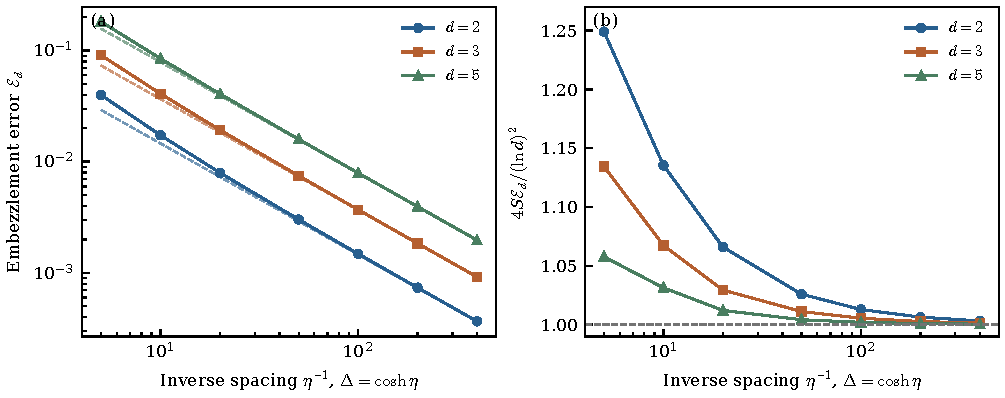
\includegraphics[width=\textwidth]{fig_xxz.pdf}
\caption{The XXZ corner-transfer-matrix spectrum in the symmetry-broken convention.
(a) The error for targets $d=2,3,5$, computed with exact integer
level multiplicities. Dashed curves show $3\eta(\ln d)^2/\pi^2$.
(b) The product $4S\mathcal E_d/(\ln d)^2$ approaches one.
Moving right sends $\eta=\operatorname{arcosh}\Delta$ to zero.
The omitted rank tail contributes less than $10^{-15}$ at each point.
The plotted values use floating-point evaluation.}
\label{fig:xxz}
\end{figure}

\begin{proposition}[Wick violation in the XXZ N\'eel phases]
\label{prop:xxz-nonquasifree}
For $1<\Delta\le21/20$, the Jordan--Wigner fermion state of each
boundary-selected N\'eel phase violates the gauge-invariant Wick identity
on two neighboring sites.
\end{proposition}

\begin{proof}
The two boundary limits of Ref.~\cite[Proposition~1.3]{ADW20} are
$U(1)$-invariant because the finite ground vectors have definite total
$Z$ spin. The staggered $Z$ rotation in their Eq.~(1.20) leaves $Z_j$
unchanged and conjugates translation to translation followed by a uniform
$Z$ rotation. Thus one-site translation still exchanges the two phases
in the convention of $H_\Delta$. Global spin flip exchanges the boundary
fields and hence the limiting states. It leaves the bond Hamiltonian
invariant and sends the even Jordan--Wigner hopping operator
$a_j^*a_{j+1}$ to its adjoint. Consequently the local $Z$ expectations
alternate between $m$ and $-m$, the bond energy $e_\Delta$ is independent
of the bond, and $|\omega(a_j^*a_{j+1})|=\alpha$ is also independent of
the bond.

Put $\eta=\operatorname{arcosh}\Delta$. In the finite-volume loop
representation of these same states~\cite[Theorem~4.2 and
Eqs.~(4.7)--(4.10)]{ADW20}, condition on the unoriented loops. The two
orientations of the loop through a site have probabilities
$e^{\pm\eta}/(e^\eta+e^{-\eta})$, with the signs exchanged for the
opposite boundary condition. Reversing that orientation flips the
site's Pauli $Z$ value. Thus the conditional mean has absolute value
$\tanh\eta$. Averaging and taking the boundary limits give
$m^2\le\tanh^2\eta=1-\Delta^{-2}$.

On an interval of $N$ sites, the fermionic covariance is a positive
contraction. A diagonal unitary makes all nearest off-diagonal
entries equal to $\alpha$. Its trace against the open-chain adjacency
matrix is then $2(N-1)\alpha$, at most the sum of the positive adjacency
eigenvalues. These are the positive members of
$2\cos(k\pi/(N+1))$, $1\le k\le N$. Dividing by $2(N-1)$ and taking
the limit gives $\alpha\le1/\pi$.

The bond energy equals the thermodynamic ground energy per site.
To see this, let $H_I$ be the open Hamiltonian of an interval $I$,
let $B_I$ be the two bonds crossing its boundary, and reset $I$ to
an open-chain ground vector. Summing the ground-state condition
$\omega(A^*[H_\Delta,A])\ge0$ over the reset channel's Kraus operators
gives $\omega(H_I)\le E_0(H_I)+2\|B_I\|$. The reverse bound is
variational. At $\Delta=1$ the exact Pauli-normalized energy is
$e_1=1-4\log2$~\cite{Hulthen38}. An $SU(2)$-averaged finite isotropic
ground state gives one third of its isotropic energy to each spin
component. Using it as a trial state for $H_\Delta$ and taking the
thermodynamic limit gives $e_\Delta\le e_1(\Delta+2)/3$.

The number relation $Z_j=2a_j^*a_j-1$ gives the Wick prediction
$\omega(Z_jZ_{j+1})=-m^2-4\alpha^2$. The hopping term has expectation
at least $-4\alpha$. The actual defect in the Wick identity therefore
satisfies
\begin{align*}
 \Delta\bigl(\omega(Z_jZ_{j+1})+m^2+4\alpha^2\bigr)
 &\le e_1(\Delta+2)/3+4/\pi+4\Delta/\pi^2+\Delta-\Delta^{-1}\\
 &\le \frac{61}{60}(1-4\log2)+\frac4\pi
       +\frac{21}{20}\left(\frac4{\pi^2}+\frac{41}{441}\right)<0.
\end{align*}
The first bound increases with $\Delta$ because $e_1>-3$. The last
strict inequality follows, for example, from $\log2>0.6931$ and
$\pi>3.1415$. The $U(1)$ symmetry sets the anomalous two-point
expectations to zero, so the defect excludes quasifreeness.
\end{proof}

\subsection{Critical bulk Hamiltonians obtained by local circuits}
\label{sec:bulk-circuits}

There is also an exact critical bulk construction at fixed coupling.
Write $h_j=(X_jX_{j+1}+Y_jY_{j+1})/2$. Controlled-phase gates turn
the XX interaction into density-dependent hopping throughout the chain.
Two choices distinguish preservation of the algebraic type from
preservation of the entire finite-chain Schmidt spectrum.

\begin{theorem}[Critical interacting bulk circuits]\label{thm:bulk-circuit}
The one-spin translation-invariant, finite-range interaction
\[
 H_{\mathrm{bulk}}=\sum_{j\in\mathbb Z}Z_{j-1}h_jZ_{j+2}
\]
has a pure gapless ground state whose physical half-chain factors are
type $\IIIone$ and satisfy Haag duality. The value of $G$ is one at
every vector in its ground-state sector. For its open finite-volume
circuit ground states, the Bell-pair embezzlement error tends to zero
and the game value tends to one.

The period-two bulk interaction
\[
 H_{\mathrm{pair}}=\sum_{j\in\mathbb Z}
 \bigl(h_{2j+1}+Z_{2j+1}h_{2j+2}Z_{2j+4}\bigr)
\]
has the same type and gaplessness properties. At the cut between $0$
and $1$, it has exactly the XX ground state's game value and
nonattainment property. On centred open intervals of $4m$ spins its
Schmidt spectrum equals that of the XX chain. Consequently every
finite-chain embezzlement law of Theorem~\ref{thm:xx-full-law} holds
unchanged for these interacting ground states.
\end{theorem}

\begin{proof}
Let $C_{j,j+1}=\operatorname{diag}(1,1,1,-1)$ on neighbouring spins.
Conjugation by this gate sends $X_j$ and $Y_j$ to $X_jZ_{j+1}$ and
$Y_jZ_{j+1}$, respectively, and fixes both $Z$ operators. The gate
commutes with $h_j$. The product over all bonds defines an involutive
automorphism $\alpha$: the gates commute and can be applied in two
layers of disjoint bonds. It commutes with one-site translation and
satisfies
\[
 \alpha(h_j)=Z_{j-1}h_jZ_{j+2}.
\]
The state $\omega_{\mathrm{XX}}\circ\alpha$ is a pure ground state
of the conjugate dynamics. Its GNS Hamiltonian is unitarily equivalent
to the XX GNS Hamiltonian and is therefore gapless.

At the cut, all gates except $C_{0,1}$ act separately in the two
halves. Thus $\alpha=\operatorname{Ad}(C_{0,1})\circ
(\alpha_L\otimes\alpha_R)$. Proposition~\ref{prop:factor} shows that
the represented half-chain pair is simultaneously unitarily conjugate
to the XX pair. Its type, Haag duality and sector-wide value one follow.
In a finite interval, conjugate the open XX Hamiltonian by the product
of its internal bond gates. The resulting Hamiltonian agrees with
$H_{\mathrm{bulk}}$ except for its boundary terms. Its ground state
converges locally to $\omega_{\mathrm{XX}}\circ\alpha$. Finite-support
approximations to the latter state's embezzling unitaries and game
measurements, as in the proof of Theorem~\ref{thm:value}, transfer both
limiting assertions to the finite intervals.

For $H_{\mathrm{pair}}$, apply the gates only on the pairs
$\{2j+1,2j+2\}$. They fix the hopping within each pair and dress the
interpair hopping by the two displayed $Z$ factors. No gate crosses
the indicated cut. The automorphism preserves both half-chain
algebras, and each finite-volume circuit is a tensor product of a
left and a right unitary. This preserves every Schmidt coefficient,
every state-specific game value, and whether its supremum is attained.
\end{proof}

These interactions contain genuine higher-order terms in the original
Jordan--Wigner fermions: the dressed hopping is multiplied by
$(1-2n_{j-1})(1-2n_{j+2})$, producing quartic and sextic terms.
Their exact circuit equivalence to XX explains why their critical
spectral laws can be transferred without approximation. The XXZ CTM
calculation supplies a different family of spectra to which the same
counting criterion applies.

\subsection{A quartic impurity in the XX representation}

Write $a(f)$ for the fermionic annihilator smeared with
$f\in\ell^2(\mathbb Z)$. Let $h$ be the single-particle nearest-neighbour
hopping operator $(h f)_j=f_{j-1}+f_{j+1}$, and let $\delta_j$ denote a
site basis vector. Put
\[
 f= h\delta_0/\sqrt2,\qquad g=h\delta_1/\sqrt2,\qquad
 V=a^*(f)a(f)a^*(g)a(g).
\]
The two vectors are orthonormal. Thus $V$ is a self-adjoint projection.
It is even and its Jordan--Wigner image $V_{\rm s}$ is a spin operator
supported on $[-1,2]$. Let $H_\lambda$ denote the spin XX interaction
perturbed by $\lambda V_{\rm s}$, where $\lambda\in\mathbb R$.

\begin{theorem}[A pure ground state in the XX sector]\label{thm:impurity}
For $0<|\lambda|<1/\sqrt8$, $H_\lambda$ has a pure ground state in the
unperturbed XX GNS representation, distinct from the original ground state.
Its two physical half-chains are type $\III$ factors in Haag duality. The
ground-state GNS Hamiltonian has positive spectrum accumulating at zero.
In particular the value of the game $G$ is one in this ground state
and at every vector in its sector, by Theorem~\ref{thm:value} and its sector-wide proof.
\end{theorem}

\begin{corollary}[A ground state that violates the quasifree description]\label{cor:nongaussian}
For $0<|\lambda|<\bigl(\frac12-\frac{4}{3\pi}\bigr)^2/(4\sqrt8)$, the ground state in
Theorem~\ref{thm:impurity} can be chosen gauge invariant with a pure,
nonquasifree Jordan--Wigner fermionic state.
\end{corollary}

\begin{corollary}[Finite impurity chains]\label{cor:impurity-finite}
Under the coupling hypothesis of Theorem~\ref{thm:impurity}, every local
subsequential limit of the centred even-length open-chain ground states is
a pure ground state in the XX sector. Their finite-chain game value tends
to one for the game $G$. Their Bell-pair embezzlement error also tends to zero.
\end{corollary}

The choice $f=h\delta_0/\sqrt2$, $g=h\delta_1/\sqrt2$ suppresses the
interaction at the Fermi points. A pull-through estimate bounds the expected
number of particle--hole excitations by $8\lambda^2$, uniformly in the
volume. This retains a nonzero overlap with the free vacuum and places an
infinite ground state in the same irreducible representation. Compactness
of the excitation vectors gives the finite-chain conclusion. The
four-excitation component of the quartic interaction then excludes a
quasifree description at small nonzero coupling. Full proofs are in
Appendix~\ref{app:interacting}.

